\documentclass[12pt,twoside]{article}

%%%%%%%%%%%%%%%%%%%%%%%%%%%%%%%%%%%%%%
% Here are commands to redefine      %
%%%%%%%%%%%%%%%%%%%%%%%%%%%%%%%%%%%%%%

\newcommand{\THISDEL}{D.1.1}
\newcommand{\THISTITLE}{First report on Work Package 1}
\newcommand{\THISPARTNER}{Trifork}


% For M12 deliverables: July 15, 2007
\newcommand{\DUEDATE}{11$^{th}$ December 2014}
\newcommand{\THISDELVERSION}{0.00}

% Dissemination level is one of
% PU (public)
% PP (program participants only)
% RE (restricted by consortium)
% CO (consortium members only)
% NB: The commission services are always included
% NB: defaults to PU
\newcommand{\THISDISSEMINATION}{CO}

%%%%%%%%%%%%%%%%%%%%%%%%%%%%%%%%%%%%%%
% End of commands to redefine        %
%%%%%%%%%%%%%%%%%%%%%%%%%%%%%%%%%%%%%%

\newcommand{\THISDATE}{\DUEDATE}

\usepackage{epsf}
\usepackage[pdftex]{graphicx}
%\usepackage{graphicx}
\usepackage{pdfpages}               % include pdf documents inside this doc
\usepackage{fancyhdr}
\usepackage{hyperref}
\usepackage{lastpage}

\setlength{\hoffset}{-10mm}
\setlength{\textwidth}{424pt}
\setlength{\voffset}{-15mm}
\setlength{\textheight}{225mm}

\hypersetup{%
	colorlinks=false,% hyperlinks will be black
	linkbordercolor=red,% hyperlink borders will be red
	pdfborderstyle={/S/U/W 1},% border style will be underline of width 1pt
	linktoc=page% defines which part of an entry in the table of contents is made into a link. Valid values: none,section,page,all
}

\pagestyle{fancy}
\fancyhead{}
\fancyfoot{}
\fancyhead[LO,RE]{\slshape\date \leftmark }
\fancyfoot[CO,CE]{\small SELFMAN Deliverable \THISDEL, \THISDATE}
\renewcommand{\headrulewidth}{0.4pt}
\renewcommand{\footrulewidth}{0.4pt}

% partners
\newcommand{\UCL}{UCL(P1)}
\newcommand{\KTH}{KTH(P2)}
\newcommand{\INRIA}{INRIA(P3)}
\newcommand{\FT}{FT R\&D(P4)}
\newcommand{\ZIB}{ZIB(P5)}
\newcommand{\NUS}{NUS(P7)}
\newcommand{\SELFMAN}{SELFMAN}


% % % % % % % % % % % % % % % % % % % % % % % % % %
% Aconyms for SyncFree project.
%
% Author: Amadeo Asco
% Last updated: 24 July 2014
% % % % % % % % % % % % % % % % % % % % % % % % % %
% The acronym package helps you manage acronyms and acronym lists in your documents, http://www.mackichan.com/index.html?techtalk/456.htm~mainFrame
% for the glossary to show up in Table of Contents you need to additionally add toc option
\usepackage[toc,nonumberlist]{glossaries}
%\showthe\hsize% interrupts latex and shows value of \hsize
\setlength{\glsdescwidth}{0.82\hsize}%
% to remove extra line between groups
\renewcommand{\glsgroupskip}{}
% To get rid of the full stop after the description in the glossary
\renewcommand{\glspostdescription}{}
\makeglossaries

% Start definitions ---------------------------
% Add all of the definitions for the abbreviations
\newacronym{2i}{2i}{Secondary Indexing}
\newacronym{2pset}{2P-Set}{Two-Phase Set}
\newacronym{acid}{ACID}{Atomicity, Consistency, Isolation, Durability}
\newacronym{b2b}{B2B}{Business to Business}
\newacronym{base}{BASE}{basically available, soft state, eventual consistency}
\newacronym{cci}{CCI}{Causality, Convergence and Intention}
\newacronym{cmrdt}{CmRDT}{Op-based Convergent Replicated Data Type}
\newacronym{cprdt}{CPRDT}{Conflict-free Partially Replicated Data Type}
\newacronym{crdt}{CRDT}{Conflict-free Replicated Data Type}
\newacronym{cqrs}{CQRS}{Command Query Responsibility Segregation}
\newacronym{cvrdt}{CvRDT}{State-based Convergent Replicated Data Type}
\newacronym{dc}{DC}{Data Centre}
\newacronym{ec}{EC}{Eventual Consistency}
\newacronym{ga}{GA}{Genetic Algorithm}
\newacronym{gset}{G-set}{State-based increment-only Counter}
\newacronym{gp}{GP}{General Practitioner}
\newacronym{ha}{HA}{High Availability}
\newacronym{id}{ID}{identifier}
\newacronym{lww}{LWW}{Last-Writer-Wins}
\newacronym{lwwr}{LWW-Register}{Last-Writer-Wins Register}
\newacronym{mdc}{MDC}{Multi Data Centre}
\newacronym{mv}{MV}{Multi-Valued}
\newacronym{mvr}{MV-Register}{Multi-Valued Register}
\newacronym{orset}{OR-set}{Observed-Removed Set}
\newacronym{rdbms}{RDBMS}{Relational Database Management System}
\newacronym{rga}{RGA}{Replicated Growing Array}
\newacronym{rest}{REST}{Representational State Transfer}
\newacronym{rpc}{RPC}{Remote Procedure Call}
\newacronym{cap}{CAP}{Consistency, Availability and Partition tolerance}
\newacronym{sec}{SEC}{Strong Eventual Consistency}
\newacronym{ttl}{TTL}{Time To Live}
\newacronym{uset}{U-Set}{Two-Phase Set with unique elements}
\newacronym{wp1}{WP1}{Work Package 1}
\newacronym{wp2}{WP2}{Work Package 2}
\newacronym{wp3}{WP3}{Work Package 3}
\newacronym{wp4}{WP4}{Work Package 4}
\newacronym{wp5}{WP5}{Work Package 5}
% end abbreviations ---------------------------

%\ifnum\showDefinitions=1
% Add all of the definitions
%\newglossaryentry{bwd}{name={box-and-whisker diagram}, text={box-and-whisker diagram}, first={box-and-whisker diagram},
%    description={\parbox{10.6cm}{\medskip The bottom and top of the box are the 25th and 75th percentile (the lower and upper quartiles, respectively), and the band near the middle of the box is the median, whereas the dot represent the mean. The ends of the whiskers represent the minimum and maximum of all of the data.\medskip}}}
% end definitions -----------------------------
%\fi

\glsdisablehyper

\makeglossaries


\begin{document}
\begin{titlepage}
\thispagestyle{fancy}
\fancyhead{}
\fancyfoot{}
\fancyfoot[CO,CE]{\small SyncFree Deliverable \THISDEL (v\THISDELVERSION), \THISDATE}
\renewcommand{\headrulewidth}{0pt}

% % Try the line below if the next line does not work for you!
% \begin{minipage}{14truecm}
% % \begin{minipage}{\textwidth}
% \begin{center}
% \begin{tabular}{lr}
% \includegraphics[height=4truecm,width=6truecm,clip=]{EVERGROW100.png} $\qquad$ & $\qquad$
% \includegraphics[height=4truecm,width=6truecm,clip=]{6fpweb2v100.png}
% \end{tabular}
% \end{center}
% \end{minipage}

\begin{center}
  
\includegraphics[width=5cm]{figures/syncfree.png} \qquad\qquad
  
\includegraphics[width=5cm]{figures/eu.jpg}
\end{center}

\vspace{3.0cm}

\begin{flushleft}
  \begin{tabular}{ll}
    Project no. & 609551 \\
    Project acronym: & SyncFree\\
    Project title: & \parbox[t]{10cm}{\noindent\it Large-scale computation without synchronisation}
  \end{tabular}
\end{flushleft}

\vspace{1.0cm}

\begin{center} \Large\bf
  European Seventh Framework Programme \\[\medskipamount]
  ICT call 10
\end{center}

\vspace{1.0cm}

\begin{flushleft}
  \begin{tabular}{ll}
    Deliverable reference number and title: & \THISDEL \\
                                            & \THISTITLE \\
    Due date of deliverable:                & \DUEDATE \\
    Actual submission date:                 & \THISDATE \\[\bigskipamount]
    Start date of project:                  & 15$^{th}$ October 2013\\
    Duration:                               & 36 months\\
    Organisation name of lead contractor \\
    for this deliverable:                   & \THISPARTNER \\
    Revision:                               & \THISDELVERSION \\
    Dissemination level:                    & \THISDISSEMINATION \\
  \end{tabular}
\end{flushleft}

\end{titlepage}

\fancyhead{}
\fancyfoot{}
\fancyhead[LO,RE]{\slshape \leftmark }
\fancyfoot[CO,CE]{\small  SyncFree Deliverable \THISDEL (v\THISDELVERSION), \THISDATE, Page \thepage}
\renewcommand{\headrulewidth}{0.4pt}

\newpage

\tableofcontents

\newpage

\renewcommand{\thepage}{\arabic{page}}
\setcounter{page}{1}

\section{Project objectives for the period} \label{s:DX-description-of-milestones}
\subsection{Overview}
% Please provide a short overview of the project objectives for the reporting period in question, as included in Annex I of the Grant Agreement. These objectives are required so that this report is a stand-alone document
The following sections provide an overview of the project objectives for the reporting period in question.

\subsubsection{D1.1 [month 6]}
Natural-language requirements: Initially, the use cases selected by the project partners will be described formally in natural language. Such a description consists of a outline of the targeted supporting architecture and a list of the informal constraints the system must ensure.

%The document can be found at \href{https://syncfree.lip6.fr/dokuwiki/lib/exe/fetch.php?media=syncfree:workpackages:wp1_d1.1_use_cases_in_natural_language.pdf}{D1.1 Delivery}.


\subsubsection{D1.2 [month 18]}
Formal-language requirements: In this task, we will describe the selected use cases using a mathematical notation suitable for reasoning, verification and computation, as required by the later Work Packages. Constraints concerning scalability, quality of service, fault tolerance, and other global guarantees will be specified qualitatively and quantitatively. This formalisation will build upon recent work on eventual consistency semantics. The behaviour and composition of data types will be defined in terms of programming models, using the first results of \gls{wp4}.


\section{Contractors contributing to the Deliverable}

\subsection{Trifork Leeds}
Amadeo Asc\'{o}, Tom Benedictus, Rune Skou Larsen and Kresten Krab Thorup.


\subsection{Ko\c{c}}
Burcu Kulahcioglu Ozkan and Serdar Tasiran.


\subsection{UNL}
Carla Ferreia.


\subsection{INRIA}
Jordi Martori Adrian, Marc Shapiro and Pascal Urso.


\subsection{KL}
Peter Zeller.


\newpage
\section{Work progress and achievements during the period} \label{s:DX-}

\subsection{Progress overview}
% Please provide a concise overview of the progress of the work and situate the main achievements in the context of the research field, including a comparative assessment with the current state of the art

%\subsection{Progress}
% For each work package -- except project management, which will be reported in section 3.5 -- please provide the following information:
%	A summary of progress towards objectives and details for each task;
%	Highlight clearly significant results; If applicable, explain the reasons for deviations from Annex I and their impact on other tasks as well as on available resources and planning

{\bf D1.1}: The ``Natural-language requirements" document was created and made available in SyncFree website, where six different use cases with their own characteristics and constraints are described using natural-language. The use cases were compiled from a group of use cases provided by the industrial partners and are described in some details in this document, also providing an outline of the informal constraints the system must ensure and the targeted supporting architecture.\\

{\bf D1.2}: ``Formal-language requirements" is not a deliverable until March 2015 (M18) but major progress has been archived. Currently there are three documents and the adaptive replication has been incorporated into this Work Package and the overall project.

All the use cases presented in D1.1 have been already modelled mathematically together with their constraints to help understanding the problem better, using a standard mathematical representation. Using this initial mathematical representation three of the six use cases have already been represented in TLA+. The TLA+ suit is well suited for concurrent and distributed systems, and it is an open-source project, which provides a language with a parser and syntax checker, model checker and simulator that will allow completing all the tasks associated with \gls{wp1}. The already represented use cases has been syntactically checked and many simulations conducted,  focusing in the verification and assurance of application-level properties for applications built using \glspl{crdt}, given that the key research question being explored by the SyncFree project is to determine the extent to which \glspl{crdt} can enable the building of practical systems.

In a \gls{wp1} meeting conducted in Paris from 9$^{th}$ to $11^{th}$ September 2014 it was agreed to be of academic and industrial interest to embrace more areas within the scope of SynchFree, particularly the study and implementation of adaptive replication.

An Adaptive Geo--replication algorithm has been proposed, described in the document "Adaptive Geo--Replication Based on Ant Colony Algorithm", and presented in M12. The algorithm is based in the well known Ant Colony algorithm commonly used in optimisation problems. An initial implementation has been provided and incorporated to a GUI application for demonstration proposes that could be further extended to allow simple tests to be carried out in a visible and controlled manner.

Five presentations were provided in M12 regarding the different areas covered up to now by \gls{wp1}.


\subsection{Progress overview and contribution to the research field}
The following sections present more information about the two deliverables covered in the pass twelve months. It must be noted that the second deliverable (D1.2) is not due in this period but main advances have been achieved which are also presented here.


\subsubsection{D1.1 - Natural language requirements}
The only deliverable for this period for \gls{wp1} corresponds to the D1.1 document with title ``Natural language requirements" which provides a general informal description in natural language of some use cases selected by the project partners, \cite{Benedictus2014a}. These use cases were selected from those originally proposed by some of the industrial partners.

Six use cases have been described by the \gls{wp1} in the SyncFree project. All use cases make use of distributed databases having one or more \glspl{dc} acting as central authority. In some use cases, the distributed database also spans to mobile devices being “sometimes connected” - both with each other and the central authority. 

A simple overview of the selected use cases is presented in Table \ref{tb:use_cases}.
\begin{table}[ht!]
	\begin{tabular}{|l|p{2.8cm}|l|p{8.1cm}|}
		\hline
		No. & Application & Provider & Brief Description \\
		\hline
		\hline
		1 & Ad Counter & Rovio & Web pages and apps are presenting commercial ads that must be displayed e.g. 100,000 times while not repeated too often on one device. \\
		\hline
		2 & Leader Board & Rovio & For each game, records must be available about the leading player. Some players use several devices. \\
		\hline
		3 & Wallet & Rovio & Debiting and keeping track of balance is is critical for a stable in-game economy. \\
		\hline
		4 & \gls{fmk} & Trifork & Sharing information on a patient’s current medication between healthcare professionals and the patient himself. \\
		\hline
		5 & \gls{b2b} & Trifork & The ability to present new products, place orders, and keep track of delivery using tablet computers is the basis for this \gls{b2b} application that connects thousands of stores with the manufacturer. \\
		\hline
		6 & Festival & Trifork & Tens of thousands of participants in one of the world’s largest two week music festivals are concurrently rating their experience and the momentary results are made generally available. \\
		\hline
	\end{tabular}
	
	\caption{Overview of selected use cases.}
	\label{tb:use_cases}
\end{table}

Another document was created with an extended discussion of the \gls{fmk} use case with the title ``Optimistic Control for a Critical System" with extra details on its current implementation and requirements, which proposes some improvements such as divergence visibility, divergence guarantees, pseudo-transactions (\glspl{crdt}) and acting on conflicts, \cite{Benedictus2014b}.


\subsubsection{D1.2 - Formal-language requirements}
This document provides a brief presentation of the natural language requirements, which shows the special nature of the paradigm shift forcing large-scale distributed applications away from \gls{rdbms}, \cite{Asco2014a}.

The document provides two mathematical representations of the use cases, and it is available in SyncFree GitHub. All use cases have been represented initially mathematically (common representation) and several of the use cases have already been represented in TLA+, syntax checked with SANY, model checked and emulated with TLC and verified. Work in progress as not all use cases has been fully represented in TLA+ and others have incomplete representations. This work is not due util M18.

The design of a dynamic behaviour exploration tool is being undertaken for applications built on top of the execution platforms developed in SyncFree, using Riak, work part of \gls{wp4}. In the process of building a tool that orchestrates multiple Riak instances running on a single machine in order to systematically explore the states that different
replicas can get into, and how this affects application-level properties.
%\href{http://research.microsoft.com/en-us/um/people/lamport/tla/tla.html}{


\subsubsection{Adaptive Replication}
It has been proposed and accepted to extend the coverage to consider Adaptive Replication. A common technique to reduce latency is the replication of data between different \glspl{dc} in a system with multiple \glspl{dc} distributed around the world, as shown in Figure \ref{fig:multi-dcs}.
\begin{figure}[ht!]
	\centering
	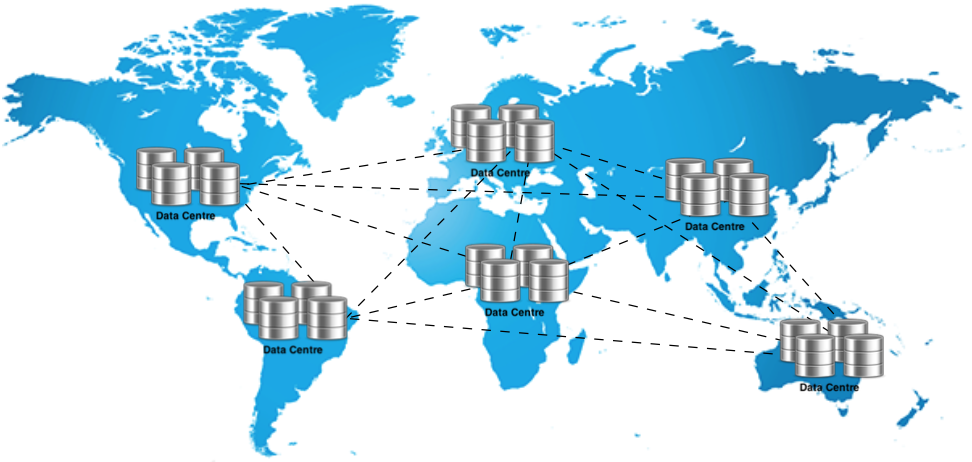
\includegraphics[width=1\textwidth]{figures/multiDCs.png}
		
	\caption{Multiple \glspl{dc} distributed around the world.}
	\label{fig:multi-dcs}
\end{figure}

But keeping multiple replicas is an expensive commodity given the increase in storage requirements and bandwidth as a write operation needs to be propagated to all the other \glspl{dc} with a replica. The data could be placed in only one \gls{dc}, in which case there is not any replication, or a copy could exist in all the available \glspl{dc}, which it is known as full replication. Alternatively the data may be located in some but not necessarily all the \glspl{dc} such that the number, location and data is determined at run time, which it is known as adaptive replication.

The replications may be grouped, base on its existence, into two types; {\bf static replication} where a replica persist until it is deleted by a user or its duration expires, and {\bf dynamic replication} where the creation and deletion of a replica are managed automatically and normally directed by the access pattern of the data used by the users \cite{Dong2008a}. In static replication the major drawback is their inability to adapt to changes in the access pattern of the data used by the users.

Also there are two types of replication based on their effect on the data; {\bf partial replication} is concerned with the number of parts the full data is composed of, all of which may be located in different parts of the overall system, i.e. \glspl{dc}, within a \gls{dc} in different nodes or at the client-side \cite{Briquemont2015a, Briquemont2014a, Serrano2007a}, whereas {\bf adaptive geo--replication} is concerned in what data and where the data or part of the data is located within the overall system of \glspl{dc} and how many replicas exist simultaneously, \cite{Jeon2014a, KingsyGrace2013a, Wang2012a, Abad2011a, Abdul-Wahid2007a, Loukopoulos2004a}.\\


{\bf Partial Replication}: 
It is concerned with the different parts of the data, \cite{Briquemont2014a, Serrano2007a}, and finding data types that allow breaking the data into smaller parts, \cite{Briquemont2015a}. It avoids replicating large data structures so helping to reduce the bandwidth and latency. The main principal is that not all the full data is always required, as shown in Figure \ref{fig:partial_replication}. This introduces the need to find data structures which allow breaking the data into parts without loosing information, and maintaining the data integrity and required invariants.
\begin{figure}[ht!]
	\centering
	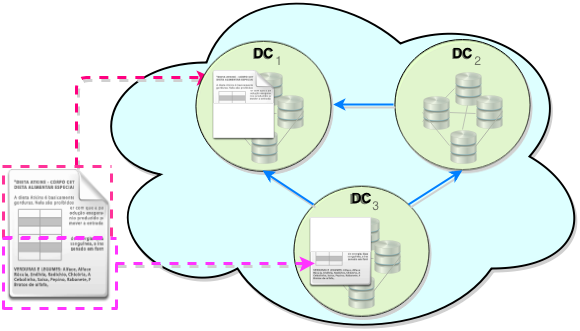
\includegraphics[width=.6\textwidth]{figures/partialReplication.png}

	\caption{Example of Partial Replication of data between multiple \glspl{dc}.}
	\label{fig:partial_replication}
\end{figure}

This requires to define new \glspl{crdt} which allows splitting the data into different parts that may be placed in multiple \glspl{dc}, \cite{Briquemont2015a}.\\


{\bf Adaptive Geo--replication}: 
This is  also know as ``Adaptive Location of Replicas". In the example, shown in Figure \ref{fig:adaptive_location_replicas}, data reads/writes to \glspl{dc} $1$ and $2$ making the data replica to move from \gls{dc} $3$ to \glspl{dc} $1$ and $2$ ensuring that the data is closer to where the reads and writes are requested based on the specified objectives and constraints.
\begin{figure}[ht!]
	\centering
	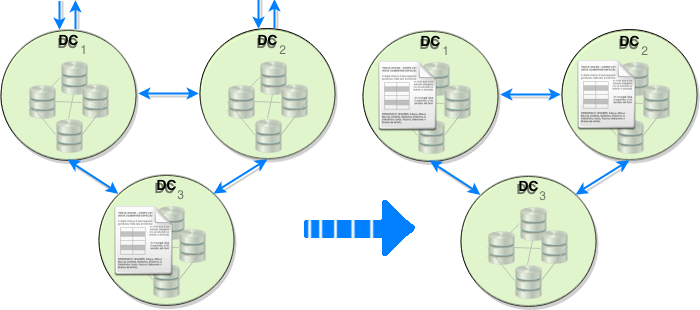
\includegraphics[width=1\textwidth]{figures/adaptiveReplication.png}
		
	\caption{Example of adaptive geo--replication between \glspl{dc}.}
	\label{fig:adaptive_location_replicas}
\end{figure}

Adaptive Geo--replication is concerned with:
\begin{enumerate}
	\item \underline{Location}: On which \glspl{dc} to place the replicas so it is
	\begin{enumerate}
		\item Improved the latency: reduce distance between user and replica,

		\item Improved the data transmission quality.
	\end{enumerate}

	\item \underline{Selection}: Which data to replicate.

	\item \underline{Number}: How many replicas to have so it is 
	\begin{enumerate}
		\item Reduced unnecessary replicas which 
		\begin{enumerate}
			\item Reduces storage consumption and

			\item Reduces required network bandwidth.
		\end{enumerate}
	\end{enumerate}
\end{enumerate}

An Initial proposal of an algorithm has been presented to the \gls{wp1} for the ``Adaptive Geo--replication". The algorithm decides without the need of human intervention where, when and how many times the data is replicated with the main objective of reducing the latency and network traffic (reduce usage of bandwidth).

In general terms any read operation in a data centre reinforces the need for a replica of the data in such \gls{dc}, similarly but perhaps with a different degree it happens with the write operations. But write operations decrease the need for a replica of the data in the other \glspl{dc} with replicas, so eventually these \glspl{dc} will not have any replica of the data. Given that we do not want to keep replicas when there are not necessary replica strength will decay as time pass, but always making sure that the data is present (replicated) at least in a pre-set number of \glspl{dc}. There is also a question about how the replication should decay as time pass, e.g. linear, exponential or arctangent.

This proposed algorithm uses simple and fast operations to adapt to the changing access pattern of the data. Furthermore, some or all of the parameters could be determined at run time by some other adaptive approach which has into account the cost function which is described in the algorithm paper.\\

This algorithm implies:
\begin{enumerate}
	\item For reads on a \gls{dc}, the \gls{dc} does not require to communicate any information to any of the other \glspl{dc}. A read only needs to use resources in the \gls{dc}, where the read is initially requested from, so no extra network traffic is imposed on the systems.

	In the particular case where a read is executed on a \gls{dc}, without a replica of the data, storage and processing power in the \gls{dc} will be required and the request will be forwarded to its closest \gls{dc} with a replica. This operation incurs in extra network traffic but if it is repeated too often the extra network traffic will be removed by replicating the data in the requesting \gls{dc} where the data was initially requested.

	\item On a write the \gls{dc} receiving the original request will (eventually) transmit it to the other \glspl{dc}, which have a replica of the data, so no need to add extra network traffic as this is the normal approach. But extra data will be sent to the other \glspl{dc} to notify them of the number of writes the changes refer to, which will depend of the type of \gls{crdt} approach used, i.e. op-based or state-based. In some cases not every write is transmitted to the other \glspl{dc}, such is the case of the state-base approach, so it would be required to keep some track of the number of merged writes.

	Also the merging of the data should only be executed after the replication strength has been calculated and when it is still higher than zero, which will reduce unnecessary operations.

	\item On data without any reads and writes on any \gls{dc}, the number of replicas will be reduced as time passes by the temporal effect, until the data is only replicated in the minimum number of \glspl{dc}.
\end{enumerate}

The algorithms has already been implemented in Java as part of a GUI tool, as shown in Figure \ref{fig:gui-tool}, that allows to easterly show its principals in a graphical manner, which was presented in the M12 meeting. The tool is available in SyncFree GitHub repository.
\begin{figure}[ht!]
	\centering
	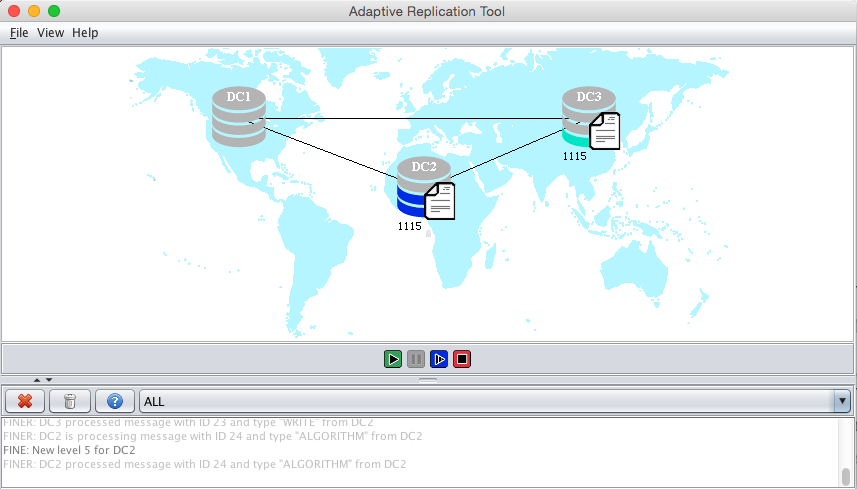
\includegraphics[width=1\textwidth]{figures/adaptiveLocationOfReplicas.png}
		
	\caption{General view of the algorithm GUI tool for three \glspl{dc}.}
	\label{fig:gui-tool}
\end{figure}
This tool also allows to run scripts, represented in XML format, which execution can be controlled by starting, stepping, pausing and stopping them. The description of the system composed of \glspl{dc} is also contained in the test script together with the operations to execute, i.e. read and write operations.

A document has been written which explains the proposed algorithm in more detail, \cite{Asco2014b}, and contains some related literature, which is available in SyncFree GitHub. Also a simple comparison has been included in the document for when there is no replication, the data is only in one \gls{dc}, when the data is fully replicated, a replica exists in all the \glspl{dc}, and when the proposed algorithm is used.\\


\subsubsection{Internet of Things}
It was presented the need to extend the scope of the overall project to cover also \gls{iot} to maintain the industrial relevance of the project up to date with the trends, technologies and emerging needs.

The \gls{iot} is a world in which machines, cloud-based applications and networked devices connect with each other, to share and process data where big data analytics facilitate intelligent decision making. It covers all verticals such as retail point of sales, automotive, asset and fleet management, healthcare, manufacturing, security, etc. Also many of the world biggest industrial players are already actively taking part in this revolution.

It is proposed to incorporate in the project two main scenarios; first of all regarding the high burst of incoming data, known as time series, and secondly referring to the listening of events which then actions must be taken upon them, known as events. So new data types are required to efficiently fulfil the requirements of these scenarios.

The work covered in \gls{wp1} regarding \gls{iot} refers to the presentation of this idea and providing the initial document with a description and some links to extra documentation and existing implementations which will be updated as further work is carried out. Also the introduction and representation of new data types are tasks for future work in \gls{wp1}.


\subsubsection{Presentations in M12}
List of presentations in M12 from \gls{wp1}.
\begin{enumerate}
	\item WP 1 Progress Overview
	\item Large Project Failure: Adaptive Replication
	\item TLA+ description and model checking
	\item Adaptive Location of Replicas: An algorithm based on the Ant Colony algorithm
	\item Shared Medical Record (FMK)
\end{enumerate}


\subsubsection{Documents}
List of current documents from \gls{wp1}.
\begin{enumerate}
	\item D1.1 Natural language requirements
	\item Optimistic Control for a Critical System
	\item Adaptive Geo–-Replication Based on Ant Colony Algorithm (work in progress)
	\item Formal Mathematical Requirements (work in progress)
\end{enumerate}


\subsubsection{Future work}
Some work to be carried out in \gls{wp1}:
\begin{enumerate}
	\item Finalise the TLA+ representations: extend to the remaining use cases and investigate the formal refinement (correct implementation) relation between a high-level \glspl{crdt} specification and a lower-level implementation, e.g. static verification (rather than model checking) of application proper ties.

	\item Run validation and simulations of the TLA+ representations.

	\item Update the algorithm document.

	\item The effort has concentrated on modelling applications that use transactions and \glspl{crdt}, but not more elaborate mechanisms for ensuring invariants such as reservations and escrow, and not more elaborate and efficient replication mechanisms such as partial or adaptive replication. Since the initial exploration of the verification and tooling issue has yielded encouraging results, it is envisage to investigate these more elaborate mechanisms, their correctness and how they enable programmers to guarantee application-wide invariants.

	\item Incorporate the algorithm in the platforms developed in SyncFree (part of \gls{wp2}) which includes the generalisation of the interface between the ``Adaptive Replication Layer" and the ``Across \glspl{dc} Replication Layer".

	\item Provide guidance on how to set the parameters in the algorithm, which should come from the test results and the study of the algorithm behaviour in different scenarios.

	\item Create papers/article regarding the algorithm and how it compares to other approaches.
	
	\item Study and propose data types for \gls{iot}.
\end{enumerate}

Other future work directly emerging from the current work curried out in \gls{wp1} are:
\begin{enumerate}
	\item Implement the algorithm in Erlang (part of \gls{wp2}) to easterly interact with the platforms developed in SyncFree.

	\item Execute comparative tests with other existing approaches present in the literature (also part of \gls{wp5}).
\end{enumerate}
	

{\bf Further work} that may be of interest:
\begin{enumerate}
	\item Extend the algorithm to use self tuning, if test results show this as appropriate, otherwise provide advise on setting the parameters based in some use cases.

	\item Extend the algorithm to consider other constraints such as the data must always be present (replicated) in a specific \gls{dc} to fulfil legal requirements.
\end{enumerate}


\subsubsection{Other work carried out}
{\bf Implementation of the proposed Adaptive Geo--replication Algorithm}\\
To help in the understanding and dissemination of the Adaptive Geo--replication algorithm principals, and as a initial prove of concept an initial implementation of the algorithm has been coded in Java but given that the algorithm was envisaged to take part in a multi layer infrastructure where the management of the replicas between \glspl{dc} is the responsibility of the ``Across \glspl{dc} Replication Layer" then a simple implementation of the ``Across \glspl{dc} Replication Layer" was implemented in Java within the tool. The ``Across \glspl{dc} Replication Layer" has already been implemented in the platforms developed in SyncFree, using Erlang programming language and Riak, and future work will be carried out to incorporate the algorithm implementation within these layers infrastructure.

A Java GUI tool has been developed which implements the algorithm and allows to test it (work in progress). The tool provides help in form of HTML files displayed on GUI components in the tool, those components may be visualised from different parts of the tool, which work as links, shown in Figure \ref{fig:tool_help}. The bottom part of the tool displays the ``log view" with the operations executed, which may be filtered to only display the messages of interest. In the middle of the display between the ``graphical view" of the replica strength progress (at the top of the GUI) and the ``log view" (at the bottom of the GUI) is the controls of the test, more information is available on the help. This tool and algorithm were coded under the scope of  \gls{wp2} and \gls{wp5}, and will be further improved and studied within the \gls{wp1}, \gls{wp2} and \gls{wp5}.
\begin{figure}[ht!]
	\centering
	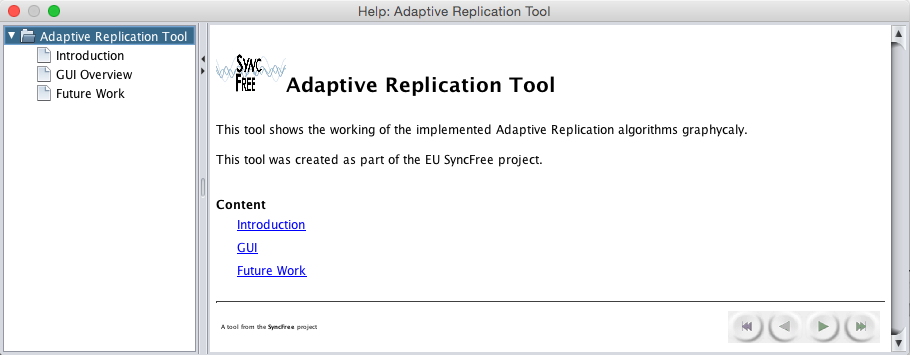
\includegraphics[width=1\textwidth]{figures/toolHelp.png}
	
	\caption{General view of the help for the Adaptive Replication Tool.}
	\label{fig:tool_help}
\end{figure}

It is intended that once the tests have been conducted to asses the algorithm performance, when compared with other algorithms, then a paper(s)/article(s) will be created in part by extending the current document with the algorithm description and incorporating the results from these tests.


\newpage
\bibliographystyle{plain}
\bibliography{../syncFree}
\printglossaries

%\newpage
\appendix
\section{Appendix}
List of documents:
\begin{itemize}
	\item \href{https://github.com/SyncFree/WP1/tree/master/D1_1/docs/wp1_D1.1_use_cases_in_natural_language.pdf}{D1.1}
	\item \href{https://github.com/SyncFree/WP1/blob/master/OCCSDoc/CriticalOptimisticEventualConsistency_0.1.pdf}{Critical Optimistic Eventual Consistency}
	\item \href{https://github.com/SyncFree/WP1/blob/master/AdaptiveReplication/docs/adaptiveAntReplication.pdf}{Adaptive Ant Replication (in progress)}
	\item \href{https://github.com/SyncFree/WP1/blob/master/D1.2/docs/D1_2.pdf}{D1.2 (in progress)}
\end{itemize}
%\includepdf[pages=-]{pdf/paper.pdf}

\end{document}
